\documentclass[11pt]{article}
\usepackage[letterpaper,margin=1in]{geometry}
\usepackage{amsmath,amssymb,amsthm}
\usepackage{lmodern}
\usepackage[T1]{fontenc}
\usepackage{tikz}
\usepackage{booktabs}
\usepackage{enumitem}
\usepackage[hidelinks]{hyperref}

\setlist{itemsep=2pt,topsep=4pt}
\numberwithin{equation}{section}
\theoremstyle{definition}
\newtheorem{example}{Example}[section]
\newtheorem{definition}{Definition}[section]
\theoremstyle{remark}
\newtheorem*{remark}{Remark}

\newcommand{\dft}{\xrightarrow{\ \text{DFT}\ }}
\newcommand{\ft}{\;\overset{\mathcal F}{\longleftrightarrow}\;}
\newcommand{\cconv}{\circledast}

\title{\textbf{Signals, Systems, and the Discrete Fourier Transform}\\[4pt]
\large Review Notes for 6.3000 Quiz 2 (Fall 2026)}
\author{Lectures of October 8 through October 29 and Homework 5--8}
\date{}

\begin{document}
\maketitle
\begin{abstract}
\noindent These notes cover everything after Quiz 1: systems and their properties (linearity and time
invariance), the unit-sample response and convolution, frequency response and filtering,
communication systems (modulation), the discrete Fourier transform, and circular convolution.
Each section develops the ideas, states the results that are used again and again, and works
examples taken from lecture, homework, and past quizzes. Quiz 2 is cumulative, so Section~1
first collects the Fourier tools from the first half of the course that this material depends on.
\end{abstract}

\tableofcontents
\newpage

%======================================================================
\section{Conventions and the Fourier Toolkit}
%======================================================================

Throughout, $t$ is continuous time and $n$ is discrete time (an integer). The variable $\omega$
is continuous-time angular frequency (rad/s) and $\Omega$ is discrete-time angular frequency
(rad/sample). The course places the normalization $1/T$ or $1/N$ in the \emph{analysis}
equations of the series and of the DFT, so that the zeroth coefficient is always the average
value of the signal.

\subsection{Five Fourier representations}
\begin{align}
\text{CTFS:}\quad & a_k=\frac1T\int_T f(t)\,e^{-jk\omega_0t}\,dt, &
 f(t)&=\sum_{k=-\infty}^{\infty}a_k e^{jk\omega_0 t}, \quad \omega_0=\tfrac{2\pi}{T},\\
\text{DTFS:}\quad & a_k=\frac1N\sum_{n=\langle N\rangle} f[n]\,e^{-jk\Omega_0n}, &
 f[n]&=\sum_{k=\langle N\rangle}a_k e^{jk\Omega_0n}, \quad \Omega_0=\tfrac{2\pi}{N},\\
\text{CTFT:}\quad & X(\omega)=\int_{-\infty}^{\infty}x(t)\,e^{-j\omega t}\,dt, &
 x(t)&=\frac1{2\pi}\int_{-\infty}^{\infty}X(\omega)\,e^{j\omega t}\,d\omega,\\
\text{DTFT:}\quad & X(\Omega)=\sum_{n=-\infty}^{\infty}x[n]\,e^{-j\Omega n}, &
 x[n]&=\frac1{2\pi}\int_{2\pi}X(\Omega)\,e^{j\Omega n}\,d\Omega,\\
\text{DFT:}\quad & X[k]=\frac1N\sum_{n=0}^{N-1}x[n]\,e^{-j\frac{2\pi}{N}kn}, &
 x[n]&=\sum_{k=0}^{N-1}X[k]\,e^{j\frac{2\pi}{N}kn}.
\end{align}
The DTFT is periodic in $\Omega$ with period $2\pi$; the DTFS and DFT coefficients are periodic
in $k$ with period $N$. A periodic signal has a Fourier transform made of impulses at its
harmonics: $f(t)\ft\sum_k 2\pi a_k\,\delta(\omega-k\omega_0)$.

\subsection{Properties that do most of the work}
Table~\ref{tab:props} lists the properties used in nearly every Quiz~2 problem. Each has a
counterpart for the other representations; the DFT versions are in Section~6.

\begin{table}[h]
\centering
\begin{tabular}{@{}lll@{}}
\toprule
Property & Time domain & Frequency domain \\
\midrule
Linearity & $a x_1+b x_2$ & $aX_1+bX_2$\\
Time shift & $x(t-t_0)$ & $e^{-j\omega t_0}X(\omega)$\\
Frequency shift & $e^{j\omega_c t}x(t)$ & $X(\omega-\omega_c)$\\
Modulation & $x(t)\cos\omega_ct$ & $\tfrac12X(\omega-\omega_c)+\tfrac12X(\omega+\omega_c)$\\
Scaling & $x(at)$ & $\tfrac1{|a|}X(\omega/a)$\\
Time reversal & $x(-t)$ & $X(-\omega)$\\
Differentiation & $\frac{d}{dt}x(t)$ & $j\omega X(\omega)$\\
Multiplication by $t$ & $t\,x(t)$ & $j\,\frac{d}{d\omega}X(\omega)$\\
Convolution & $(x*h)(t)$ & $X(\omega)H(\omega)$\\
Multiplication & $x(t)\,h(t)$ & $\tfrac{1}{2\pi}(X*H)(\omega)$\\
Conjugate symmetry & $x$ real & $X(-\omega)=X^*(\omega)$\\
Parseval & $\int|x|^2dt$ & $\frac1{2\pi}\int|X|^2d\omega$\\
\bottomrule
\end{tabular}
\caption{Fourier transform properties (CT notation; the DTFT is identical with $\Omega$, $n$, and
$\frac1{2\pi}\int_{2\pi}$).}
\label{tab:props}
\end{table}

Two symmetry facts save a great deal of algebra:
a real, even signal has a real, even transform; a real, odd signal has an imaginary, odd
transform. A pure delay never changes the magnitude of a transform.

%======================================================================
\section{Systems}
%======================================================================

A \emph{system} is any process that transforms an input signal into an output signal. We write
$x\to y$, or draw a box labeled $S$ between $x[n]$ and $y[n]$. Examples range from a three-point
averager,
\begin{equation}
y[n]=\tfrac13\big(x[n-1]+x[n]+x[n+1]\big),
\end{equation}
which smooths noisy data, to an audio equalizer or a cell-phone channel. Arbitrary systems are
arbitrarily hard to describe, but most useful systems share two properties, linearity and time
invariance, and for those systems the theory is complete.

\subsection{Linearity}
\begin{definition}
A system is \emph{additive} if the response to a sum of inputs is the sum of the responses:
if $x_1\to y_1$ and $x_2\to y_2$, then $x_1+x_2\to y_1+y_2$, for all inputs.
It is \emph{homogeneous} if scaling the input scales the output: $\alpha x\to\alpha y$ for every
constant $\alpha$ and every input. A system that is both additive and homogeneous is
\emph{linear}; equivalently, $\alpha x_1+\beta x_2\to\alpha y_1+\beta y_2$.
\end{definition}

Homogeneity with $\alpha=0$ shows that a linear system must map the zero input to the zero
output. This gives the fastest test for nonlinearity: if $x=0$ produces $y\neq0$, the system is
neither additive nor homogeneous. Trying $\alpha=-1$ catches systems such as $|x[n]|$.

\subsection{Time invariance}
\begin{definition}
A system is \emph{time-invariant} if delaying the input delays the output by the same amount:
if $x[n]\to y[n]$ then $x[n-n_0]\to y[n-n_0]$ for all $n_0$ and all inputs.
\end{definition}

To test it, compute the response to the shifted input, $\tilde y[n]$, and compare it with the
shifted output $y[n-n_0]$. Time invariance fails whenever the time index appears outside the
argument of $x$ (as in $n\,x[n]$ or $x[n]\cos\omega n$), or the argument of $x$ is altered
(as in $x[-n]$ or $x[2n]$).

\begin{example}[Spring 2025 Quiz 2]
Classify four systems.
\begin{enumerate}[label=(\alph*)]
\item $y[n]=\left(-\frac12\right)^n\big(x[n]+1\big)$. With $x_1+x_2$ the output is
$\left(-\frac12\right)^n(x_1+x_2+1)\neq y_1+y_2$, so it is not additive; with $\alpha x$ it is
$\left(-\frac12\right)^n(\alpha x+1)\neq\alpha y$, so it is not homogeneous. The shifted input gives
$\left(-\frac12\right)^n(x[n-m]+1)$, while $y[n-m]=\left(-\frac12\right)^{n-m}(x[n-m]+1)$:
not time-invariant. Answer: No, No, No.
\item $y[n]=\sin(x[n])$: $\sin(x_1+x_2)\ne\sin x_1+\sin x_2$ and $\sin(\alpha x)\ne\alpha\sin x$,
but the system acts sample by sample with no reference to $n$. Answer: No, No, Yes.
\item $y(t)=\int_{-\infty}^t x(\tau)\,d\tau$: integration is linear, and substituting
$\lambda=\tau-t_0$ shows $\int_{-\infty}^t x(\tau-t_0)d\tau=\int_{-\infty}^{t-t_0}x(\lambda)d\lambda
=y(t-t_0)$. Answer: Yes, Yes, Yes.
\item $y(t)=t\,x(t)$: linear, but $t\,x(t-t_0)\ne(t-t_0)x(t-t_0)$. Answer: Yes, Yes, No.
\end{enumerate}
\end{example}

\subsection{Difference and differential equations}
A system described by a linear difference equation with constant coefficients,
\begin{equation}
\sum_{k}a_k\,y[n-k]=\sum_k b_k\,x[n-k],
\label{eq:diffeq}
\end{equation}
and started from rest (all signals zero before the input begins), is linear and time-invariant:
a weighted sum of solutions is a solution, and a delayed solution is a solution. The same holds
for linear differential equations with constant coefficients,
$\sum_k a_k \frac{d^k y}{dt^k}=\sum_k b_k\frac{d^kx}{dt^k}$.
A constant term (such as $y[n]=x[n]+1$) or a coefficient that depends on $n$ breaks this.

An LTI system has three equivalent descriptions, and the rest of these notes moves between them:
\begin{enumerate}
\item a difference (or differential) equation: algebraic constraints on samples;
\item the unit-sample (or impulse) response $h$: the output for a unit-sample input;
\item the frequency response $H$: how each frequency is scaled and phase-shifted.
\end{enumerate}

%======================================================================
\section{Unit-Sample Response and Convolution}
%======================================================================

\subsection{Signals as sums of shifted unit samples}
The unit sample $\delta[n]$ is 1 at $n=0$ and 0 elsewhere. Any DT signal is a weighted sum of
shifted unit samples,
\begin{equation}
x[n]=\sum_{k=-\infty}^{\infty}x[k]\,\delta[n-k].
\end{equation}
Let $h[n]$ be the response of an LTI system to $\delta[n]$ (the \emph{unit-sample response}).
Time invariance gives $\delta[n-k]\to h[n-k]$, homogeneity gives $x[k]\delta[n-k]\to x[k]h[n-k]$,
and additivity sums the pieces:
\begin{equation}
\boxed{\;y[n]=\sum_{k=-\infty}^{\infty}x[k]\,h[n-k]\equiv(x*h)[n].\;}
\label{eq:conv}
\end{equation}
This is \emph{convolution}. The unit-sample response is a complete description of an LTI
system: knowing $h$, the output for any input follows. Convolution acts on whole signals; the
6.3000 notation $(x*h)[n]$ emphasizes that $x*h$ is a new signal evaluated at $n$.

\subsection{Two ways to compute a convolution}
\paragraph{Superposition.} Add shifted copies of $x$, each scaled by a sample of $h$ (or the
reverse, since convolution is commutative). A table keeps the bookkeeping straight.

\begin{example}[superposition table]
Let $x[n]=1$ for $0\le n\le3$ and $h=[1,2,3]$ starting at $n=0$.
\begin{center}
\begin{tabular}{@{}l*{8}{r}@{}}
\toprule
$n$ & 0 & 1 & 2 & 3 & 4 & 5 & 6 & 7\\
\midrule
$h[0]\,x[n]$ & 1 & 1 & 1 & 1 & 0 & 0 & 0 & 0\\
$h[1]\,x[n-1]$ & 0 & 2 & 2 & 2 & 2 & 0 & 0 & 0\\
$h[2]\,x[n-2]$ & 0 & 0 & 3 & 3 & 3 & 3 & 0 & 0\\
\midrule
$(x*h)[n]$ & 1 & 3 & 6 & 6 & 5 & 3 & 0 & 0\\
\bottomrule
\end{tabular}
\end{center}
\end{example}

\paragraph{Flip and shift.} To get one output sample, flip $h$ to form $h[-k]$, slide it right by
$n$ to form $h[n-k]$, multiply pointwise with $x[k]$, and sum. This view is best when you need
a single value or a closed form.

\subsection{Properties of convolution}
\begin{align}
x*h&=h*x &&\text{(commutative)}\\
(x*h_1)*h_2&=x*(h_1*h_2) &&\text{(associative)}\\
x*(h_1+h_2)&=x*h_1+x*h_2 &&\text{(distributive)}\\
x*\delta&=x,\qquad (x*\delta_{n_0})[n]=x[n-n_0] &&\text{(identity and shift)}
\end{align}
Here $\delta_{n_0}[n]=\delta[n-n_0]$. Associativity means a cascade of systems has
$h=h_1*h_2$ (in either order); distributivity means a parallel connection has $h=h_1+h_2$.
Two bookkeeping rules help check answers. If $x$ is nonzero only on $[a_1,b_1]$ and $h$ only on
$[a_2,b_2]$, then $x*h$ is nonzero only on $[a_1+a_2,\,b_1+b_2]$; for finite sequences of lengths
$L_1$ and $L_2$ the result has length $L_1+L_2-1$. And sums multiply:
$\sum_n(x*h)[n]=\big(\sum x\big)\big(\sum h\big)$, which is the statement $Y(0)=X(0)H(0)$.

\subsection{Results worth knowing by heart}
With $u[n]$ the unit step,
\begin{align}
(u*u)[n]&=(n+1)\,u[n], &
(u*u*u)[n]&=\frac{(n+1)(n+2)}{2}\,u[n],\\
(a^nu[n]*u[n])&=\frac{1-a^{n+1}}{1-a}\,u[n], &
(a^nu[n]*b^nu[n])&=\frac{a^{n+1}-b^{n+1}}{a-b}\,u[n]\ (a\ne b).
\end{align}
Two equal pulses of length $L$ convolve to a triangle of length $2L-1$ with peak $L$.

\begin{example}[Spring 2025 Quiz 2, cascaded systems]
A system with $h_1=u$ driven by $x[n]=0.9^nu[n]$ gives
$y_1[n]=\sum_{m=0}^{n}0.9^m=10-9(0.9)^n$, whose first values are $1,\ 1.9,\ 2.71,\ 3.439,\ 4.0951$.
Cascading three accumulators gives $h_{123}=u*u*u$, with values $1,3,6,10,15$.
\end{example}

\begin{example}[Fall 2022 Quiz 2]
Let $f_1[n]=(-1)^n$ for $0\le n<6$. Every product in $(f_1*f_1)[n]$ is
$(-1)^m(-1)^{n-m}=(-1)^n$, so the result is $(-1)^n$ times the overlap count:
\[
(f_1*f_1)[n]=1,\,-2,\,3,\,-4,\,5,\,-6,\,5,\,-4,\,3,\,-2,\,1\qquad(0\le n\le10).
\]
\end{example}

\subsection{Continuous time}
The impulse $\delta(t)$ is the limit of a pulse of width $\Delta$ and height $1/\Delta$. Writing
$x(t)=\int x(\tau)\delta(t-\tau)\,d\tau$ and repeating the argument above gives the
\emph{convolution integral}
\begin{equation}
y(t)=(x*h)(t)=\int_{-\infty}^{\infty}x(\tau)\,h(t-\tau)\,d\tau,
\end{equation}
where $h(t)$ is the \emph{impulse response}. Evaluate it piecewise: sketch $x(\tau)$ and the
flipped, shifted $h(t-\tau)$, and integrate the product over each range of $t$ where the overlap
has the same form.

\begin{example}
Two unit pulses $p(t)=1$ on $0<t<1$ give a triangle: $(p*p)(t)=t$ for $0\le t\le1$ and $2-t$
for $1\le t\le2$. For $h(t)=e^{-t}u(t)$ and $x=u$,
$y(t)=\int_0^t e^{-\tau}d\tau=(1-e^{-t})u(t)$.
\end{example}

\begin{remark}
Derivatives move freely: $(x*h)'=x'*h=x*h'$. When one signal is piecewise constant, its
derivative is a set of impulses, and convolving with impulses only shifts and scales copies of
the other signal. This is the quickest way through the convolution-matching problems.
\end{remark}

\subsection{Finding the unit-sample response}
For a difference equation, run the recursion with $x=\delta$ from rest. For
$y[n]-\frac12y[n-1]=x[n]$: $h[0]=1$, $h[1]=\frac12$, $h[2]=\frac14$, and in general
$h[n]=\left(\frac12\right)^nu[n]$. Going the other way, an infinite sum often collapses into a short
recursion: $h[n]=\sum_{i\ge0}\alpha^i\delta[n-4i]$ gives $y[n]=x[n]+\alpha x[n-4]+\dots$, and
subtracting $\alpha y[n-4]$ leaves $y[n]-\alpha y[n-4]=x[n]$ (Fall 2022 Quiz 2).

%======================================================================
\section{Frequency Response and Filtering}
%======================================================================

\subsection{Complex exponentials are eigenfunctions}
Feed $x[n]=e^{j\Omega n}$ into an LTI system:
\begin{equation}
y[n]=\sum_k h[k]\,e^{j\Omega(n-k)}=\Big(\sum_k h[k]e^{-j\Omega k}\Big)e^{j\Omega n}=H(\Omega)\,e^{j\Omega n}.
\end{equation}
The output is the same complex exponential, multiplied by the complex number
\begin{equation}
\boxed{\;H(\Omega)=\sum_{n}h[n]\,e^{-j\Omega n},\;}
\end{equation}
the \emph{frequency response}, which is the DTFT of the unit-sample response. In continuous time,
$e^{j\omega t}\to H(\omega)e^{j\omega t}$ with $H(\omega)=\int h(t)e^{-j\omega t}dt$.

Since $\cos\Omega n=\frac12e^{j\Omega n}+\frac12e^{-j\Omega n}$ and $H(-\Omega)=H^*(\Omega)$ for a real
$h$, a sinusoid comes out as a scaled, phase-shifted sinusoid of the same frequency:
\begin{equation}
\cos(\Omega_0 n)\;\longrightarrow\;|H(\Omega_0)|\cos\!\big(\Omega_0n+\angle H(\Omega_0)\big)
=\operatorname{Re}H\,\cos\Omega_0n-\operatorname{Im}H\,\sin\Omega_0n.
\label{eq:sinusoid}
\end{equation}
The last form answers questions of the type ``write $y[n]=A\cos\Omega_0n+B\sin\Omega_0n$''.

\subsection{Convolution in time is multiplication in frequency}
Because every input is a superposition of complex exponentials, and each is simply scaled,
\begin{equation}
y=x*h\quad\Longleftrightarrow\quad Y(\Omega)=X(\Omega)\,H(\Omega).
\end{equation}
This is the filtering view: each frequency component of the input is scaled by $|H|$ and
shifted in phase by $\angle H$. A cascade multiplies frequency responses; a parallel connection
adds them. It also gives system identification: if an LTI system maps $x$ to $y$, then
$H=Y/X$ wherever $X\ne0$.

\subsection{From a difference equation to a rational frequency response}
Taking the DTFT of \eqref{eq:diffeq} term by term ($x[n-k]\to e^{-j\Omega k}X$) gives
\begin{equation}
H(\Omega)=\frac{Y(\Omega)}{X(\Omega)}=\frac{\sum_k b_ke^{-j\Omega k}}{\sum_k a_ke^{-j\Omega k}}.
\end{equation}
For $y[n]-\alpha y[n-1]=x[n]$ with $|\alpha|<1$, $H(\Omega)=1/(1-\alpha e^{-j\Omega})$, which
matches the DTFT of $h[n]=\alpha^nu[n]$. Three methods give the same answer: transform $h$,
substitute $x=e^{j\Omega n}$ and $y=He^{j\Omega n}$, or transform the equation.
In continuous time, $\tau y'(t)+y(t)=x(t)$ gives $H(\omega)=1/(1+j\omega\tau)$.

\subsection{Reading magnitude and phase}
\begin{itemize}
\item $H(0)=\sum_n h[n]$ is the DC gain; $H(\pi)=\sum_n(-1)^nh[n]$ is the gain at the highest DT
frequency.
\item Treat $1-\alpha e^{-j\Omega}$ as the difference of two vectors in the complex plane: as $\Omega$
goes from 0 to $\pi$ its length goes from $1-\alpha$ to $1+\alpha$. So $1/(1-\alpha e^{-j\Omega})$
with $0<\alpha<1$ is a low-pass filter (gain $\frac1{1-\alpha}$ at DC, $\frac1{1+\alpha}$ at $\pi$),
and with $-1<\alpha<0$ it is high-pass.
\item A phase that is linear in $\Omega$ with slope $-d$ is a delay by $d$ samples. Factor the
delay out to expose a real amplitude:
\begin{equation}
1-e^{-j2\Omega}=e^{-j\Omega}\big(e^{j\Omega}-e^{-j\Omega}\big)=j\,2\sin(\Omega)\,e^{-j\Omega}.
\end{equation}
\item A jump of $\pi$ in the phase is a sign change of the real amplitude, not a delay.
\end{itemize}

\begin{example}[Spring 2025 and Spring 2022 Quiz 2]
For $g[n]=\delta[n]-\delta[n-2]$, $G(\Omega)=j\,2\sin(\Omega)e^{-j\Omega}$: the magnitude is
$2|\sin\Omega|$ (zero at $0$ and $\pm\pi$, peak 2 at $\pm\frac\pi2$); the phase is
$\frac\pi2-\Omega$ on $0<\Omega<\pi$ and jumps by $\pi$ wherever $\sin\Omega$ changes sign, giving a
sawtooth between $\pm\frac\pi2$.
\end{example}

\begin{example}[Spring 2022 Quiz 2]
Let $h[n]=\left(\frac12\right)^n$ for even $n\ge0$ and 0 otherwise. Then
$H(\Omega)=\sum_{m\ge0}4^{-m}e^{-j2m\Omega}=\dfrac{1}{1-\frac14e^{-j2\Omega}}$. At
$\Omega=\frac\pi4$, $e^{-j\pi/2}=-j$, so $H=\frac{1}{1+j/4}=\frac{16-4j}{17}$, and by
\eqref{eq:sinusoid} the input $\cos(\pi n/4)$ produces
$\frac{16}{17}\cos\frac{\pi n}{4}+\frac4{17}\sin\frac{\pi n}{4}$.
\end{example}

\begin{example}[cascade of first-order systems]
Three subsystems $y_i+y_i'=x_i$ in cascade have $H(\omega)=(1+j\omega)^{-3}$. At $\omega=1$,
$\frac{1}{1+j}=\frac{1}{\sqrt2}e^{-j\pi/4}$, so $\cos t\to\frac{1}{2\sqrt2}\cos\!\big(t-\frac{3\pi}{4}\big)$.
\end{example}

\begin{example}[Fall 2022 Quiz 2, system identification]
Cascading $h_1=e^{-t}u(t)$ and $h_2=e^{-2t}u(t)$ gives
$H=\frac{1}{(1+j\omega)(2+j\omega)}$, so $\big(2+3j\omega+(j\omega)^2\big)Y=X$, that is
$2y+3y'+y''=x$.
\end{example}

\begin{example}[Fall 2023 Quiz 2, finding the system]
An LTI system maps $x_1[n]=2^{-n/2}u[n]$ to $\delta[n]$. Then
$H_1=\frac{1}{X_1}=1-\frac{1}{\sqrt2}e^{-j\Omega}$, with magnitude rising from $1-\frac1{\sqrt2}$ at
$\Omega=0$ to $1+\frac1{\sqrt2}$ at $\Omega=\pi$.
\end{example}

\subsection{Ideal filters}
An ideal low-pass filter passes $|\Omega|<\Omega_c$ with gain 1 and blocks the rest of
$(-\pi,\pi]$. Its unit-sample response is
\begin{equation}
h[n]=\frac1{2\pi}\int_{-\Omega_c}^{\Omega_c}e^{j\Omega n}d\Omega=\frac{\sin\Omega_cn}{\pi n},
\qquad h[0]=\frac{\Omega_c}{\pi}.
\end{equation}
It is infinitely long and non-causal, so it cannot be built exactly; real filters approximate it.
A high-pass filter is $1-H_{\text{LP}}$ on the same band edges. Filtering a sum of sinusoids
is then a matter of keeping or deleting each one, and scaling the survivors by $H$.

%======================================================================
\section{Communication Systems}
%======================================================================

\subsection{Matching the signal to the medium}
Telephone-quality speech spans roughly 200--3000\,Hz. An antenna should be comparable to a
wavelength, and $\lambda=c/f$ is 100--1500\,km at these frequencies, which is absurd. The cure is
to move the message to a band that suits the medium. Modulation does this, and nearly every
communication scheme is built on it.

\subsection{Multiplication in time is convolution in frequency}
The dual of the convolution property is
\begin{equation}
y(t)=x(t)\,c(t)\quad\Longleftrightarrow\quad Y(\omega)=\frac{1}{2\pi}(X*C)(\omega).
\end{equation}
For a carrier $c(t)=\cos\omega_ct$, $C(\omega)=\pi\delta(\omega-\omega_c)+\pi\delta(\omega+\omega_c)$,
and convolving with an impulse just places a copy:
\begin{equation}
x(t)\cos\omega_ct\ \ft\ \tfrac12X(\omega-\omega_c)+\tfrac12X(\omega+\omega_c).
\end{equation}
Multiplying by $e^{j\omega_ct}$ alone would shift $X$ up, but the result would be complex; the
cosine shifts one copy up and one down and keeps the signal real. This is
\emph{amplitude modulation} (AM): the message modulates the amplitude of the carrier.

\begin{figure}[h]
\centering
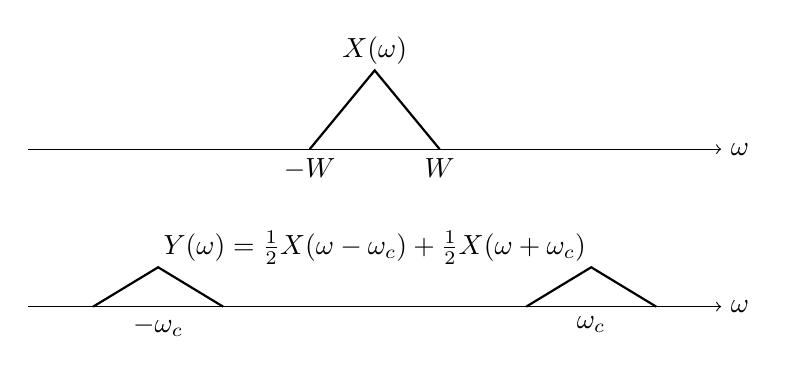
\begin{tikzpicture}[x=0.55cm,y=1cm]
 % X(omega)
 \draw[->] (-8,0)--(8,0) node[right]{$\omega$};
 \draw[thick] (-1.5,0)--(0,1)--(1.5,0);
 \node at (0,1.25) {$X(\omega)$}; \node[below] at (1.5,0) {$W$}; \node[below] at (-1.5,0) {$-W$};
 % Y(omega)
 \begin{scope}[yshift=-2cm]
 \draw[->] (-8,0)--(8,0) node[right]{$\omega$};
 \draw[thick] (3.5,0)--(5,0.5)--(6.5,0); \draw[thick] (-6.5,0)--(-5,0.5)--(-3.5,0);
 \node at (0,0.75) {$Y(\omega)=\frac12X(\omega-\omega_c)+\frac12X(\omega+\omega_c)$};
 \node[below] at (5,0) {$\omega_c$}; \node[below] at (-5,0) {$-\omega_c$};
 \end{scope}
\end{tikzpicture}
\caption{Spectrum of a band-limited message and of the AM signal $y(t)=x(t)\cos\omega_ct$.}
\end{figure}

If $X(\omega)=0$ for $|\omega|>W$, the modulated spectrum occupies $\omega_c-W\le|\omega|\le\omega_c+W$,
a bandwidth of $2W$. The two copies do not overlap as long as $\omega_c>W$.

\subsection{Synchronous demodulation}
Multiply the received signal by the carrier again:
\begin{equation}
z(t)=x(t)\cos^2\omega_ct=\tfrac12x(t)+\tfrac12x(t)\cos2\omega_ct.
\end{equation}
The first term is the message at half amplitude; the second sits around $\pm2\omega_c$, starting at
$2\omega_c-W$. A low-pass filter with gain 2 and cutoff anywhere in $W<\omega_{co}<2\omega_c-W$
recovers $x(t)$ exactly.

\paragraph{Phase error.} If the receiver's carrier is $\cos(\omega_ct+\phi)$,
\begin{equation}
x(t)\cos\omega_ct\cos(\omega_ct+\phi)=\tfrac12x(t)\cos\phi+\tfrac12x(t)\cos(2\omega_ct+\phi),
\end{equation}
so the recovered message is scaled by $\cos\phi$; at $\phi=\pi/2$ it vanishes entirely. The receiver
must know the carrier's phase.

\subsection{AM with a carrier and envelope detection}
Sending the carrier along with the message, $y(t)=\big(x(t)+C\big)\cos\omega_ct$, shifts the DC value of
the message. If $C\ge\max|x(t)|$, the envelope $x(t)+C$ never changes sign and can be recovered with
a simple rectifier and smoother, with no synchronization. The cost is power: the carrier term carries
no information. This is acceptable for broadcast radio but not for battery-powered point-to-point
links. For $y=(1+\cos\omega_mt)\cos\omega_ct$, only $\frac13$ of the average power is in the sidebands.

\subsection{Frequency-division multiplexing}
Several messages can share one medium if their modulated spectra do not overlap: each uses its own
carrier, and a receiver selects one with a band-pass filter around its carrier. Three 4\,kHz
messages with DSB AM need $3\times8$\,kHz plus any guard bands.

%======================================================================
\section{The Discrete Fourier Transform}
%======================================================================

\subsection{Why another Fourier representation}
The DTFS is limited to periodic signals. The DTFT handles any signal but needs an infinite sum and
gives a function of the continuous variable $\Omega$, which a computer cannot store. The DFT takes
a finite portion of a signal, $N$ samples, and returns $N$ numbers at discrete frequencies:
\begin{equation}
X[k]=\frac1N\sum_{n=0}^{N-1}x[n]\,e^{-j\frac{2\pi}{N}kn},\qquad
x[n]=\sum_{k=0}^{N-1}X[k]\,e^{j\frac{2\pi}{N}kn}.
\end{equation}
The formulas are those of the DTFS. The difference is the interpretation: for the DTFS, $N$ is the
period of the signal; for the DFT, $N$ is simply the length of the window we analyze.
$X[0]$ is the average of the $N$ samples, and $X[k]$ is periodic in $k$ with period $N$, so
$X[N-k]$ represents the negative frequency $-k$.

\subsection{Two ways to read the DFT}
\paragraph{Periodic extension (DTFS view).} The $N$-point DFT of $x[n]$ equals the DTFS of the
signal obtained by repeating the window $x[0],\dots,x[N-1]$ forever. If a signal really is
periodic with period $N$, the DFT and DTFS coefficients agree: $\cos(2\pi n/64)$ analyzed with $N=64$
gives exactly $X[1]=X[63]=\frac12$. But $\cos(3\pi n/64)$ has period 128, not 64; its periodic
extension has a jump at the window boundary, and many coefficients are needed to build that jump.

\paragraph{Sampled DTFT of a windowed signal (DTFT view).} Let $w[n]=1$ for $0\le n<N$ and
$x_w[n]=x[n]w[n]$. Then
\begin{equation}
\boxed{\;X[k]=\frac1N\,X_w\!\left(\frac{2\pi k}{N}\right),\;}
\end{equation}
the DFT samples the DTFT of the windowed signal at $N$ equally spaced frequencies in $[0,2\pi)$ and
scales by $\frac1N$. Sampling and scaling are harmless; the windowing is what matters.

\subsection{Windowing and leakage}
The window's DTFT is
\begin{equation}
W(\Omega)=\sum_{n=0}^{N-1}e^{-j\Omega n}=e^{-j\Omega\frac{N-1}{2}}\,\frac{\sin(N\Omega/2)}{\sin(\Omega/2)},
\end{equation}
a periodic sinc with peak $N$ at $\Omega=0$ and zeros at multiples of $2\pi/N$; the main lobe is
$4\pi/N$ wide. For a windowed exponential $e^{j\Omega_0n}w[n]$ the DTFT is $W(\Omega-\Omega_0)$, a copy of
the window spectrum centered at $\Omega_0$. Sampling it at $\Omega=2\pi k/N$:
\begin{itemize}
\item if $\Omega_0=2\pi m/N$ (an integer number of cycles fits the window), one sample lands on the
peak and every other sample lands on a zero: a single clean bin;
\item otherwise no sample lands on a zero, and energy appears in every bin. This is \emph{leakage}.
\end{itemize}
A real cosine on bin $m$ gives $X[m]=X[N-m]=\frac12$ and zero elsewhere; a cosine half-way between
bins gives two equal largest bins and a slowly decaying spread.

\begin{figure}[h]
\centering
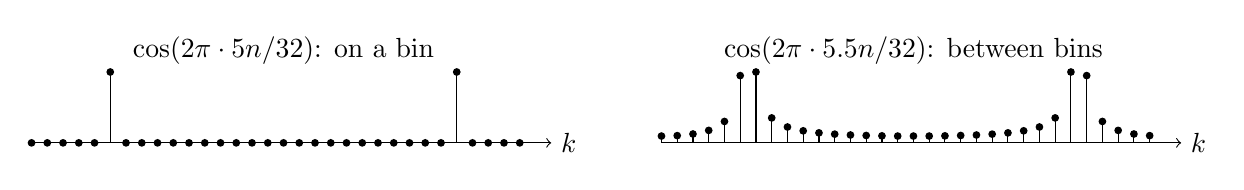
\begin{tikzpicture}[x=0.2cm,y=0.9cm]
 \draw[->] (0,0)--(33,0) node[right]{$k$};
 \foreach \k in {0,...,31} { \pgfmathsetmacro{\v}{(\k==5 || \k==27) ? 1 : 0} \draw (\k,0)--(\k,\v); \fill (\k,\v) circle (1.4pt); }
 \node at (16,1.3) {$\cos(2\pi\cdot5n/32)$: on a bin};
 \begin{scope}[xshift=8cm]
 \draw[->] (0,0)--(33,0) node[right]{$k$};
 % |X[k]| normalized to peak 1, computed with numpy for cos(2*pi*5.5*n/32)
 \foreach \k/\v in {0/0.096,1/0.102,2/0.125,3/0.176,4/0.302,5/0.949,6/1.000,7/0.352,8/0.224,9/0.170,10/0.141,11/0.123,12/0.111,13/0.104,14/0.099,15/0.096,16/0.096,17/0.096,18/0.099,19/0.104,20/0.111,21/0.123,22/0.141,23/0.170,24/0.224,25/0.352,26/1.000,27/0.949,28/0.302,29/0.176,30/0.125,31/0.102} {
   \draw (\k,0)--(\k,\v); \fill (\k,\v) circle (1.4pt); }
 \node at (16,1.3) {$\cos(2\pi\cdot5.5n/32)$: between bins};
 \end{scope}
\end{tikzpicture}
\caption{Sketch of $|X[k]|$ for a 32-point DFT of a cosine on a bin (left) and half-way between
bins (right, leakage).}
\end{figure}

\subsection{Frequency resolution}
Bin $k$ corresponds to $\Omega_k=2\pi k/N$, that is, to $f_k=kf_s/N$ hertz when the samples are taken
at $f_s$. The bin spacing is $f_s/N$, and the window lasts $N/f_s$ seconds. A peak at bin $k$ only
locates a frequency to within about one bin.

\begin{example}[the cello note from lecture]
A recording at $f_s=44{,}100$\,Hz analyzed with $N=1024$ has its largest bin at $k=7$, that is
$7\times44100/1024\approx301.5$\,Hz, with an uncertainty of $\pm f_s/N\approx\pm21.5$\,Hz. That cannot
tell D ($293.7$\,Hz) from E-flat ($311.1$\,Hz). With $N=32{,}768$ the spectrum shows two separate peaks
near $292$ and $307$\,Hz: both notes are present.
\end{example}

Resolution improves only with a longer window of real data. Padding with zeros samples the same
$X_w(\Omega)$ more densely, which makes plots smoother, but it does not separate frequencies that
the window length cannot separate. Shorter windows give better time resolution and worse frequency
resolution; the short-time Fourier transform (after this quiz) trades one for the other.

\subsection{Properties of the DFT}
All indices are taken modulo $N$.
\begin{align}
x[(n-n_0)\bmod N]&\dft e^{-j\frac{2\pi}{N}kn_0}X[k] &&\text{(circular shift)}\\
e^{j\frac{2\pi}{N}k_0n}x[n]&\dft X[(k-k_0)\bmod N] &&\text{(modulation)}\\
(-1)^nx[n]&\dft X[(k-\tfrac N2)\bmod N] &&\text{($N$ even)}\\
x[(-n)\bmod N]&\dft X[(-k)\bmod N] &&\text{(reversal)}\\
x\text{ real}&\ \Rightarrow\ X[N-k]=X^*[k] &&\text{(conjugate symmetry)}\\
\tfrac1N\textstyle\sum_n|x[n]|^2&=\textstyle\sum_k|X[k]|^2 &&\text{(Parseval, 6.3000 convention)}
\end{align}
For example, $\delta[n-1]$ with $N=4$ has $X[k]=\frac14e^{-j\pi k/2}$, so $X[1]=-\frac j4$.

\subsection{Closing sums}
Almost every DFT calculation reduces to a finite geometric sum,
\begin{equation}
\sum_{n=0}^{N-1}e^{-j\frac{2\pi}{N}mn}=\frac{1-e^{-j2\pi m}}{1-e^{-j2\pi m/N}}=
\begin{cases}N,& m\text{ a multiple of }N,\\ 0,&\text{otherwise.}\end{cases}
\end{equation}
The numerator is always zero; the answer is $N$ only where the denominator also vanishes, which is
resolved by noting that every term of the sum equals 1. Thus (Spring 2022 Quiz 2) for $0\le k<N$:
$\sum_ne^{-j2\pi kn/N}=N\delta[k]$, $\sum_ne^{j2\pi k_0n/N}e^{-j2\pi kn/N}=N\delta[k-k_0]$, and
$\sum_ne^{-j4\pi kn/N}=N\delta[k]+N\delta[k-\frac N2]$.

\begin{example}[Fall 2022 Quiz 2, DFTs of sinusoids, $N=32$]
Write each frequency as $2\pi m/32$ and ask whether $m$ is an integer.
$\cos(9\pi n/16)$ has $m=9$: two clean spikes at $k=9$ and $23$.
$\cos(9\pi n/36)=\cos(\pi n/4)$ has $m=4$: clean spikes at 4 and 28.
$\cos(9\pi n/32)$ has $m=4.5$: leakage around 4.5 and 27.5.
$\cos^2\theta=\frac12+\frac12\cos2\theta$ turns $\cos^2(9\pi n/32)$ into a DC spike plus bins 9 and 23.
$\cos^3\theta=\frac34\cos\theta+\frac14\cos3\theta$ leaks around $4.5$ and $13.5$.
\end{example}

%======================================================================
\section{Circular Convolution}
%======================================================================

\subsection{What multiplying DFTs does}
For the DTFT, a product of transforms is a convolution in time. For the DFT the same calculation
runs into a difficulty: the signals only exist for $0\le n<N$, and the exponentials
$e^{j2\pi kn/N}$ are periodic in $n$. Carrying out the algebra for $F[k]=F_a[k]F_b[k]$ gives
\begin{equation}
f[n]=\frac1N\sum_{m=0}^{N-1}f_b[m]\,f_a[(n-m)\bmod N]\equiv\frac1N(f_a\cconv f_b)[n],
\end{equation}
so with the 6.3000 convention
\begin{equation}
\boxed{\;F_a[k]\,F_b[k]\ \longleftrightarrow\ \tfrac1N\,(f_a\cconv_N f_b)[n].\;}
\end{equation}
Multiplying DFTs is circular convolution in time, with an extra factor $\frac1N$.

\subsection{Computing a circular convolution}
Circular convolution is ordinary convolution followed by \emph{time aliasing}:
\begin{enumerate}
\item compute the linear convolution $f_a*f_b$;
\item add every sample at $n\ge N$ onto $n\bmod N$ (wrap the tail around);
\item the result is periodic with period $N$.
\end{enumerate}
Continuing the earlier example, $[1,1,1,1]*[1,2,3]=[1,3,6,6,5,3]$:

\begin{center}
\begin{tabular}{@{}l*{6}{r}@{}}
\toprule
$N$ & \multicolumn{6}{l}{one period of $f_a\cconv_N f_b$}\\
\midrule
6 & 1 & 3 & 6 & 6 & 5 & 3\\
5 & 4 & 3 & 6 & 6 & 5 & \\
4 & 6 & 6 & 6 & 6 & & \\
3 & 7 & 8 & 9 & & & \\
2 & 12 & 12 & & & & \\
1 & 24 & & & & & \\
\bottomrule
\end{tabular}
\end{center}
For $N=1$ everything piles onto one sample: the product of the sums, $4\times6=24$.

\subsection{When circular equals linear}
If $f_a$ has length $L_1$ and $f_b$ has length $L_2$, their linear convolution has length $L_1+L_2-1$.
Nothing wraps when $N\ge L_1+L_2-1$, and then circular convolution equals linear convolution. This is
how convolution is computed in practice: zero-pad both signals to such an $N$, take DFTs, multiply,
and invert (with an FFT this is far faster than the direct sum).

\begin{example}[Fall 2023 Quiz 2]
Let $f[n]=1$ for $5\le n\le9$ and let $g_N$ have DFT $F_N[k]^2$. The linear convolution $f*f$ is a
triangle on $10\le n\le18$ with values $1,2,3,4,5,4,3,2,1$ (peak at $n=14$). Then
$g_N=\frac1N(f\cconv_Nf)$:
\begin{itemize}
\item $N=15$: samples at $15,\dots,18$ (values $4,3,2,1$) wrap to $0,\dots,3$:
$g_{15}[0..4]=\frac1{15}(4,3,2,1,0)$;
\item $N=12$: samples at $12,\dots,18$ wrap to $0,\dots,6$: $g_{12}[0..4]=\frac1{12}(3,4,5,4,3)$;
\item $N=10$: samples at $10,\dots,18$ wrap to $0,\dots,8$: $g_{10}[0..4]=\frac1{10}(1,2,3,4,5)$.
\end{itemize}
The same signal also gives $F(0)=5$, $F(\pi/2)=\sum_{n=5}^{9}(-j)^n=-j$, and $F(\pi)=-1$.
\end{example}

\begin{example}[Fall 2022 Quiz 2]
$g_1[n]$ is 1 on even samples and 0 on odd ones; with $N=6$ the window holds $1,0,1,0,1,0$. Then
$N\cdot\mathrm{IDFT}(G_1^2)$ is the 6-point circular self-convolution. The linear result is
$1,0,2,0,3,0,2,0,1$; wrapping $n=6,8$ onto $0,2$ gives $3,0,3,0,3,0$.
\end{example}

%======================================================================
\section{Strategies for Quiz Problems}
%======================================================================

\paragraph{System tables.} Test zero input first (a nonzero output kills additivity and
homogeneity). Then try $\alpha=-1$. For time invariance, look for a stray $n$ or $t$, or an altered
argument of $x$.

\paragraph{Transform-property matching.} For each derived signal write the transform in terms of
$F$: scaling stretches or compresses, a delay leaves the magnitude unchanged, modulation by
$e^{\pm j\omega_0t}$ shifts one copy, $\cos$ and $\sin$ create two copies that add or subtract (so
$\sin$ modulation is zero at $\omega=0$), $f*f$ squares the magnitude (sharper lobes), and $t\,f(t)$
differentiates (zero wherever $F$ is flat, such as $\omega=0$ for an even pulse).

\paragraph{DFT matching.} Decide on-bin versus off-bin first. Then use symmetry: real signals have
$|X[k]|=|X[N-k]|$; real even signals have real DFTs; sines have imaginary DFTs (real part zero);
$\delta[n-n_0]$ has constant magnitude $\frac1N$ and phase $-2\pi kn_0/N$.

\paragraph{Convolution problems.} Track support and area first; they rule out most candidates.
Use superposition tables for short sequences and the derivative trick for piecewise-constant CT
signals.

\paragraph{Frequency response.} Factor out linear phase, evaluate at $\Omega=0$, $\frac\pi2$, $\pi$
to anchor sketches, and remember that a sinusoid through an LTI system only changes amplitude and
phase.

\paragraph{Circular convolution.} Do the linear convolution, wrap, and remember the factor $\frac1N$
whenever the problem multiplies DFTs computed with the 6.3000 convention.

\appendix
%======================================================================
\section{Reference Tables}
%======================================================================

\begin{table}[h]
\centering
\begin{tabular}{@{}ll@{}}
\toprule
Signal & Transform\\
\midrule
$\delta(t)$, $\ \delta(t-t_0)$ & $1$, $\ e^{-j\omega t_0}$\\
$1$, $\ e^{j\omega_0t}$ & $2\pi\delta(\omega)$, $\ 2\pi\delta(\omega-\omega_0)$\\
$e^{-at}u(t)$, $a>0$ & $\dfrac{1}{a+j\omega}$\\[4pt]
$1$ for $|t|<T_1$ & $\dfrac{2\sin\omega T_1}{\omega}$\\[4pt]
$1-|t|$ for $|t|<1$ & $\left(\dfrac{\sin(\omega/2)}{\omega/2}\right)^2$\\[4pt]
$\dfrac{\sin Wt}{\pi t}$ & 1 for $|\omega|<W$\\
\midrule
$\delta[n-n_0]$ & $e^{-j\Omega n_0}$\\
$a^nu[n]$, $|a|<1$ & $\dfrac{1}{1-ae^{-j\Omega}}$\\[4pt]
$1$ for $0\le n<L$ & $e^{-j\Omega\frac{L-1}2}\dfrac{\sin(L\Omega/2)}{\sin(\Omega/2)}$\\[4pt]
$e^{j\Omega_0n}$ & $2\pi\sum_m\delta(\Omega-\Omega_0-2\pi m)$\\
\midrule
$\delta[n-n_0]$ ($N$-point DFT) & $\frac1Ne^{-j2\pi kn_0/N}$\\
$e^{j2\pi k_0n/N}$ ($N$-point DFT) & $\delta[(k-k_0)\bmod N]$\\
\bottomrule
\end{tabular}
\caption{Transform pairs.}
\end{table}

\paragraph{Fourier series of common waveforms} (period $T$, $\omega_0=2\pi/T$):
a pulse of duty $D$ centered at $t=0$ has $a_k=\dfrac{\sin\pi kD}{\pi k}$ and $a_0=D$;
the $\pm1$ square wave has $a_k=\dfrac{2}{j\pi k}$ for odd $k$ and 0 for even $k$;
the 0-to-1 sawtooth has $a_0=\frac12$ and $a_k=\dfrac{j}{2\pi k}$;
the 0-to-1 triangle has $a_0=\frac12$ and $a_k=\dfrac{2}{\pi^2k^2}$ for odd $k$;
$|\sin(\pi t/T)|$ has $a_k=\dfrac{2}{\pi(1-4k^2)}$.

\paragraph{Identities.}
$\cos\theta=\frac{e^{j\theta}+e^{-j\theta}}2$, $\sin\theta=\frac{e^{j\theta}-e^{-j\theta}}{2j}$,
$\sum_{n=0}^{N-1}z^n=\frac{1-z^N}{1-z}$, $\sum_{n\ge0}z^n=\frac{1}{1-z}$ for $|z|<1$,
$\cos^2\theta=\frac12+\frac12\cos2\theta$, $\cos^3\theta=\frac34\cos\theta+\frac14\cos3\theta$,
$2\cos a\cos b=\cos(a-b)+\cos(a+b)$.

\paragraph{Sampling.} $x[n]=x(nT_s)$ maps $\omega$ to $\Omega=\omega T_s=2\pi f/f_s$. DT frequencies are
only defined modulo $2\pi$, so a tone at $f$ is indistinguishable from one at $|f-mf_s|$. To avoid
aliasing, sample faster than twice the highest frequency.

\end{document}
